% Chapter Template

\chapter{Sistemas de Detección de Intrusiones} % Main chapter title

\label{Chapter2} % Change X to a consecutive number; for referencing this chapter elsewhere, use \ref{ChapterX}

%----------------------------------------------------------------------------------------
%	SECTION 1
%----------------------------------------------------------------------------------------

\section{Qué son los IDS}
Tal y como se ha visto en el capítulo anterior, la llegada de Internet y su extensión en todo tipo de ámbitos ha supuesto, además de un gran avance, la introducción de ciertos riesgos y vulnerabilidades, antes inexistentes. A día de hoy resulta inconcebible que una empresa de cierto tamaño no cuente con su propia red o utilice Internet para llevar a cabo gran parte de su actividad. Las facilidades que esta apertura al exterior puede proporcionar se contraponen con los ataques que estas organizaciones son susceptibles de sufrir. Pese a que existen soluciones que tratan de garantizar la seguridad y que únicamente los usuarios autorizados accedan a los recursos, dichas soluciones no resultan infalibles y dependen, además, de tareas de mantenimiento que están sujetas a fallos u olvidos. Es ahí donde entran en juego los IDS o  sistemas de detección de intrusiones\cite{Kemmerer}.
Una vez que el atacante ha traspasado las medidas de prevención resulta esencial detectarlo por las siguientes razones:
\begin{itemize}
	\item Cuanto antes se localice la intrusión, antes se pueden tomar medidas al respecto y, por lo tanto, menor será el daño causado por el ataque.
	\item De la misma manera que un sistema de alarmas instalado en una casa puede disuadir a ladrones a la hora de perpetrar un robo, un IDS también puede frenar posibles ataques.
	\item La detección de ataques proporciona una gran cantidad de información sobre las estrategias empleadas por los atacantes, y contribuyen a solventar vulnerabilidades del sistema de prevención.
\end{itemize}
En un paso previo a la descripción de los sistemas de detección de intrusiones, a continuación se explican los riesgos y los distintos ataques que puede sufrir un sistema. Dejando al margen los virus, que junto con las intrusiones representan los ataques más comunes, podrían distinguirse distintos tipos de intrusos\cite{Stallings2016}:
\begin{itemize}
	\item \textbf{Impostor}: en este caso el intruso entra en el sistema bajo la identidad de un usuario legitimo y hace uso de los recursos de dicha cuenta.
	\item \textbf{Usuario negligente}: un usuario legitimo del sistema utiliza de manera errónea o abusiva los recursos a los que tiene acceso, ya sean datos o programas.
	\item \textbf{Usuario clandestino}. Se trata de un atacante que intenta apropiarse de los privilegios del administrador o superusuario. Bajo la identidad del administrador el atacante puede, además, eludir controles de acceso o el registro de sus actividades.
\end{itemize}
%-----------------------------------
%	SUBSECTION 1
%-----------------------------------
\subsection{Tipos de IDS}
Existen dos criterios para clasificar los IDS: según dónde se coloquen o según la técnica que empleen. Atendiendo al punto de la red en que se encuentre, hay:
\begin{itemize}
	\item \textbf{IDSs basados en \textit{host} o máquina (HIDS)}: se localizan a nivel de una única máquina, corriendo como aplicaciones, y analizan ficheros de log para detectar intrusiones.
	\item \textbf{IDSs basados en red (NIDS)}: este tipo de IDS se encuentra en puntos concretos de la red, ya sea a la entrada o en el área desmilitarizada \textit{DMZ}. En este caso se analiza todo el tráfico de la red y no solamente el que llega a cierta máquina.
	\item \textbf{IDSs híbridos}: en este caso se combinan las dos modalidades previamente mencionadas.
\end{itemize}
\begin{figure}[t]
\centering
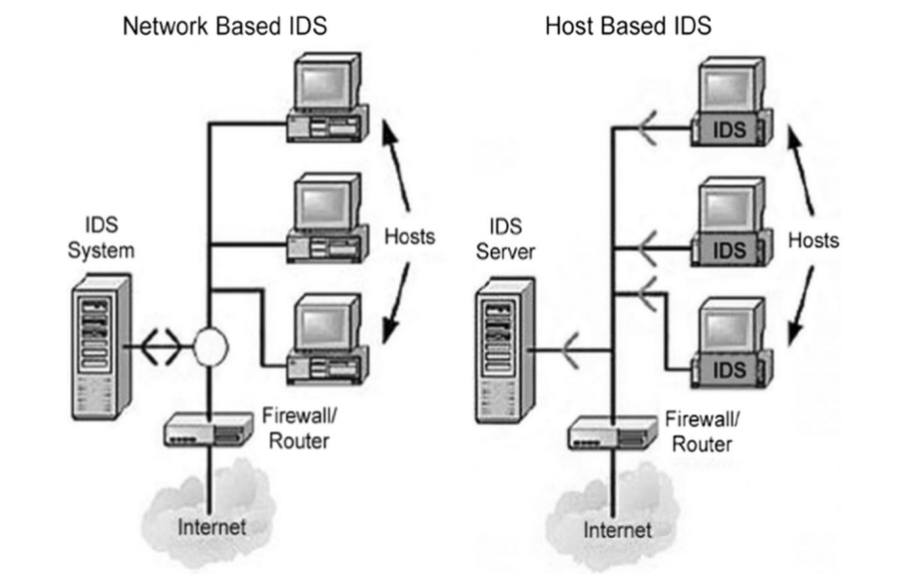
\includegraphics[width=0.9\textwidth]{images/hids.png}
\caption{Comparación entre un HIDS y un NIDS }
\label{fig:hids}
\end{figure}
Por otro, en función de la técnica que se utilice para detectar la intrusión, se encuentran los siguientes IDSs:
\begin{itemize}
	\item \textbf{Detección por uso inadecuado o basada en conocimiento}: se buscan trazas de ataques, patrones en el tráfico de red o registros en logs que puedan denotar un comportamiento sospechoso. Este tipo de sistema reconocería como sospechoso un número elevado de intentos fallidos de acceso.
	\item \textbf{Detección por firma}: En este caso, se monitorizan los paquetes de la red, comparándolos con patrones predeterminados y reconocidos, que se conocen como firmas. Ante la detección de un nuevo ataque, expertos extraen características que se traducen en firmas y permitan su detección en futuras ocasiones. Este tipo de sistemas presenta como inconveniente el lapso de tiempo que transcurre entre que se detecta un ataque y la firma está disponible.
	\item \textbf{Detección por anomalía}: la instrusión es detectada cuando se identifica un comportamiento anómalo para determinado perfil o se superan los umbrales fijados según análisis estadísticos. Algunos ejemplos de los ataques que se pueden detectar serían suplantación de la identidad o un ataque de denegación de servicio. 
\end{itemize}
\cite{Vuppala}

\subsection{Características de un IDS}
A la hora de utilizar un IDS es importante ser consciente de que se trata de una herramienta muy potente, pero pese a ello, presenta ciertas limitaciones. Es capaz, sin embargo de: 
\begin{itemize}
	\item Registrar la actividad de los usuarios.
	\item Comprobar las alteraciones y modificaciones que se producen en ciertos datos.
	\item Actualizarse para responder ante los últimos ataques.
	\item Detectar si el sistema está sufriendo un ataque.
	\item Localizar errores de configuración.
	\item Facilitar la creación de políticas de seguridad por parte del administrador.
	\item Realizar gestión de la seguridad.
\end{itemize}
Además, presenta un diseño dedicado a infraestructura, lo que supone una ventaja para implantarlo en un sistema.
No obstante, tal y como se ha mencionado, resulta importante ser consciente de ciertos inconvenientes, como la falta de solución ante mecanismos de autenticación inseguros, la necesidad de una persona que investigue los posibles ataques detectados o los problemas que presenta a la hora de analizar el tráfico en una red, cuando este es muy elevado \cite{Vuppala}.\\
A continuación en las siguientes secciones se describiran dos de los IDS más utilizados a día de hoy, \textit{Snort} y \textit{Suricata}, discutiéndose también la elección del primero para el desarrollo del proyecto.


%----------------------------------------------------------------------------------------
%	SECTION 2
%----------------------------------------------------------------------------------------

\section{Snort}
Snort se trata de un software gratuito y de código abierto desarrollado en 1998 por Martin Roesch. Desde su aparición, ha ido mejorando y extendiéndose, encontrándose consolidado como uno de los IDSs \textit{open source} más potentes y eficaces. En la actualidad el proyecto se encuentra a cargo de la empresa \textit{Sourcefire}, creada también por Martin Roesch, y que fue comprada por \textit{Cisco} en 2013. Pese al desarrollo de una versión comercial, Sourcefire 3D System, Snort sigue adelante respaldado por una amplia comunidad.\\
En lo que respecta a las funcionalidades de Snort, es posible distinguir tres modos de funcionamiento distinto:
\begin{itemize}
	\item \textbf{sniffer}: en este modo, Snort lee los paquetes que atraviesan la red y los muestra por pantalla.
	\item \textbf{Logger de paquetes}: loguea o registra los paquetes capturados en disco.
	\item \textbf{Network Intrusion Detection System}: Cuando funciona en este modo, Snort lleva a cabo tareas de análisis y detección del tráfico de la red. Este modo ofrece multitud de opciones de configuración, lo que puede suponer cierta dificultad. 
\end{itemize}
\cite{Syngress}

\subsection{Arquitectura de Snort}
Las distintas funcionalidades descritas anteriormente se implementan a través de una serie de \textit{plugins} que presenta la arquitectura modular del sistema. Snort consta de un núcleo o core con 4 módulos \cite{Shimonski}:
\begin{itemize}
	\item \textbf{\textit{Sniffer} de paquetes}: este plugin permite escuchar el tráfico que viaja a través de la red, siendo incluso posible almacenar los paquetes capturados para su posterior lectura
	\item \textbf{Decodificador}: identifica los protocolos que encapsula el paquete desde el nivel de capa de enlace hasta los niveles TCP/IP. Los paquetes atraviesan por lo tanto una cascada de decodificadores hasta que su contenido queda guardado en estructuras de datos según sus correspondientes campos. De esta manera el contenido de los paquetes queda preparado para ser tratado por los preprocesadores.
	\item \textbf{Preprocesador}: El preprocesador de snort engloba una serie de \textit{plugins} o módulos encargados de diversas tareas que facilitan y aceleran la detección en el siguiente módulo (motor de detección) al realizarse el \textit{matching} con las reglas. Se puede variar el número de preprocesadores que los paquetes han de atravesar, variando con ello también el tiempo total de procesamiento, lo que resulta fundamental a la hora de determinar la eficacia de snort.\\
Entre las funciones que pueden realizar los preprocesadores se encuentran \cite{Syngress}:
\begin{itemize}
	\item \underline{Detección de anomalías}. Consiste en determinar si el contenido de un paquete se ajusta a lo que corresponde con los protocolos que lo encapsulan.
	\item \underline{Agregación de sesiones TCP}. Este preprocesador recoge los datos de una sesión TCP, agrupándolos de manera que posteriormente sean evaluados y analizados en su conjunto. Esto se debe a que gran parte de los ataques suelen llegar en distintos fragmentos, de manera que serían indetectables si fuesen estudiados por separado.
	\item \underline{Ensamblado de fragmentos IP}. De manera similar a lo que ocurría con las sesiones TCP, los paquetes IP pueden sufrir fragmentaciones debido a las limitaciones de la red, en concreto al MTU (\textit{Maximum Transfer Unit}) que determina el tamaño máximo de un paquete para que pueda atravesar un enlace. De esta manera resulta posible que un ataque quede enmascarado en varios fragmentos y no genere ninguna alerta.
	\item \underline{Detección de escaneo de puertos}. Resulta muy difícil detectar un escaneo de puertos haciendo uso únicamente de reglas, pues hay que tener en cuenta que para realizarlo se envían paquetes a distintos hosts y puertos, en conexiones distintas. Por otro lado, existen ciertos paquetes que no cumplen las especificaciones y denotan que se esta llevando a cabo este tipo de ataque. Es el caso de un paquete \textit{NULL}
\end{itemize}
	\item \textbf{Motor de detección}. Este módulo se encarga de procesar los paquetes procedentes del preprocesador. Para ello utiliza una serie de reglas contra las que analiza los paquetes. En caso de encajar, son enviados al procesador de alertas.\\
El sistema de reglas empleado por Snort se basa en la detección mediante firmas o signatures. Este método se basa en comparar los datos de los paquetes, como cadenas, con ciertos patrones conocidos de ataques. A esta comparativa las reglas de snort añaden la posiblidad de generar expresiones de manera que se produzca una coincidencia solo bajo determinadas circunstancias. Con todo ello, este sistema resulta extremadamente rápido (gracias a la detección mediante patrones) y fiable, pues el hecho de fijar determinados parámetros permite reducir el número de falsos positivos (alertas generadas por paquetes que no constituyen ningún ataque).

	\item \textbf{Módulo de alertas y logs}. Este componente se encarga de gestionar los paquetes que hayan coincidido con alguna regla. Existen multitud de posibilidades a la hora de tratar las alertas y logs generados. Por ejemplo, se pueden guardar las alertas en ficheros en máquinas remotas haciendo uso de sockets Unix o mostrar la información referente a los logs en interfaces web. Todo ello requiere el empleo de \textit{plugins} adicionales, al igual que ocurría con los preprocesadores.
\end{itemize}
\begin{figure}[t]
\centering
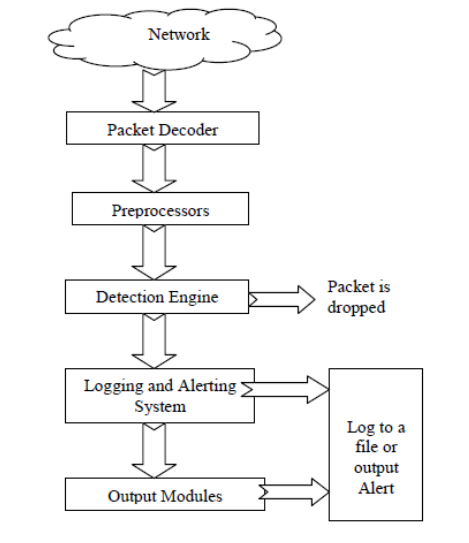
\includegraphics[width=0.5\textwidth]{images/snortArch.png}
\caption{Arquitectura de snort}
\label{fig:snortArch}
\end{figure}

\subsection{Reglas de Snort}
Las reglas de snort constituyen la clave del sistema, encontrándose agrupadas en función del tipo de ataque que detectan. Existen ya numerosas reglas en el proyecto, que pueden añadirse a Snort con un simple \textit{include} en el fichero de configuración. Pese a ello, la sintaxis simple y descriptiva del lenguaje que emplean estas reglas permite que cualquier usuario pueda escribir sus propias reglas, una vez se haya familiarizado con esta.\\
Las reglas constan de dos partes \cite{snortman}:
\begin{itemize}
	\item \textbf{Header o cabecera}. Esta primera parte contiene la acción a realizar en caso de que la regla coincida, así como, las direcciones IP y puertos, tanto de origen como destino.
	\item \textbf{Opciones}. Esta segunda parte, incluye el mensaje que ha de mostrarse en la alerta y otros parámetros adicionales, como las partes del paquete que han de evaluarse para determinar si se cumple la regla o no.
\end{itemize}
